\documentclass[a4paper,10pt]{article}

\usepackage[margin=1in]{geometry} 	% Setea el margen manualmente, todos iguales.
\usepackage[spanish]{babel} 		% {Con estos dos anda
\usepackage[utf8]{inputenc} 		% todo lo que es tildes y ñ}
\usepackage{fancyhdr} 			%{Estos dos son para
\pagestyle{fancyplain} 			% el header copado}
\usepackage{color}			% Con esto puedo hacer la matufia de poner en color blanco un texto para engañar al formato
\usepackage{xcolor,graphicx}
\usepackage{hyperref}
\usepackage{caratula}
\usepackage{algorithm}
\usepackage{algorithmic}

\lhead{Teoría de las Comunicaciones}% {Con esto se usa el header copado. También está \chead para
\rhead{Trabajo Práctico 1b} 	% el centro y comandos para el pie de página, buscar fancyhdr}


%%%%%%%%%%%%%%%%%%%%%%%%%%%%%%%%%%%%%
%      COMANDOS ÚTILES USADOS       %
%%%%%%%%%%%%%%%%%%%%%%%%%%%%%%%%%%%%%

% \section{title} 		Te hace un título ``importante'' en negrita, numerado. También está \subsection{title} y \subsubsection{title}.
% \begin{itemize}		Te hace viñetas.
%	\item esto es un item	Cambiar itemize por enumerate te hace una numeración.
% \end{itemize}

% \textbf{text} 		Te hace el texto en negrita (bold).
% \underline{text}		Te subraya el texto.

% \textsuperscript{text}	Te hace ``superindices'' con texto. En teoría subscript debería funcionar, pero se puede usar guion bajo entre llaves
% 				y signos peso para hacerlo como alternativa. Sino buscar.

% \begin{tabular}{cols} 	Es para hacer tablas. Se pone una c por cada columna deseada dentro de cols (si es que se desea centrada, l para justificar a 
%	a & b & c		izquierda, r a la derecha). Si se separa por espacios la tabla no tendrá líneas divisorias. Si se separa por | en lugar de 
% \end{tabular}			espacios, aparecerá una línea. Con || dos, y así. Luego para los elementos de las filas se escriben y se separan con ampersand (&).
%				Finalmente, para las líneas horizontales, se usa \hline para una linea en toda la tabla y \cline{i - j} te hace la linea desde
%				la celda i hasta la j, arrancando en 1.
%				Si en la columna se pone p(width) podés escribir un párrafo en la celda. Para hacer un enter con \\ no funciona porque te hace un
%				enter en la fila. Para eso se usa el comando \newline.
  
% \textcolor{color predefinido en palabras}{text}

%%%%%%%%%%%%%%%%%%%%%%%%%%%%%%%%%%%%%
%    FIN COMANDOS ÚTILES USADOS     %
%%%%%%%%%%%%%%%%%%%%%%%%%%%%%%%%%%%%%

\begin{document}

%%%%%%%%%%%%%%%%%%%%%%%%%%%%%%
%    Carátula										      %
%%%%%%%%%%%%%%%%%%%%%%%%%%%%%%

\materia{Teoría de las Comunicaciones}
\submateria{Segundo Cuatrimestre de 2013}
\titulo{Trabajo Práctico 1b - Rutas en Internet}

\grupo{Grupo 1}
\integrante{Giordano, Mauro}{125/10}{mauro.foxh@gmail.com}
\integrante{Tastzian, Juan Manuel}{039/10}{jm@tast.com.ar}
\integrante{Torres, Sebastian}{723/06}{sebatorres1987@hotmail.com}


\begin{titlepage}
\maketitle
\thispagestyle{empty}
\end{titlepage} 
\newpage

%%%%%%%%%%%%%%%%%%%%%%%%%%%%%%%%%%%%
%    Tabla de contenidos/Índice    						%
%%%%%%%%%%%%%%%%%%%%%%%%%%%%%%%%%%%%

\newpage
\tableofcontents
\newpage

%%%%%%%%%%%%%%%%%%%%%%%%%%%%%%
%    Introducción Teórica   					   %
%%%%%%%%%%%%%%%%%%%%%%%%%%%%%%

\section{Introducción}

En el presente trabajo se realiza una amplia experimentación con la capa tres del modelo OSI, es decir, con el nivel de red. A partir de un desarrollo propio de la herramienta $traceroute$ (en su versión sobre mensajes ICMP) sobre el framework Scapy para python, se colectan muestras a lo largo del día de $round-trip time$ a 3 Universidades del mundo, así como también se colectan muestras utilizando otra implementación incluida en Linux de la misma aplicación. Debido a la variabilidad de esta medición, cada experimento se repite $n$ veces para luego obtener un promedio representativo de la colección de datos. En base a la implementación de traceroute en Python, se implementa además una heurística para poder identificar enlaces transatlánticos en la ruta, lo cual es objeto de la segunda parte de experimentación de este trabajo.\\

\begin{figure}[h!]
  \centering
  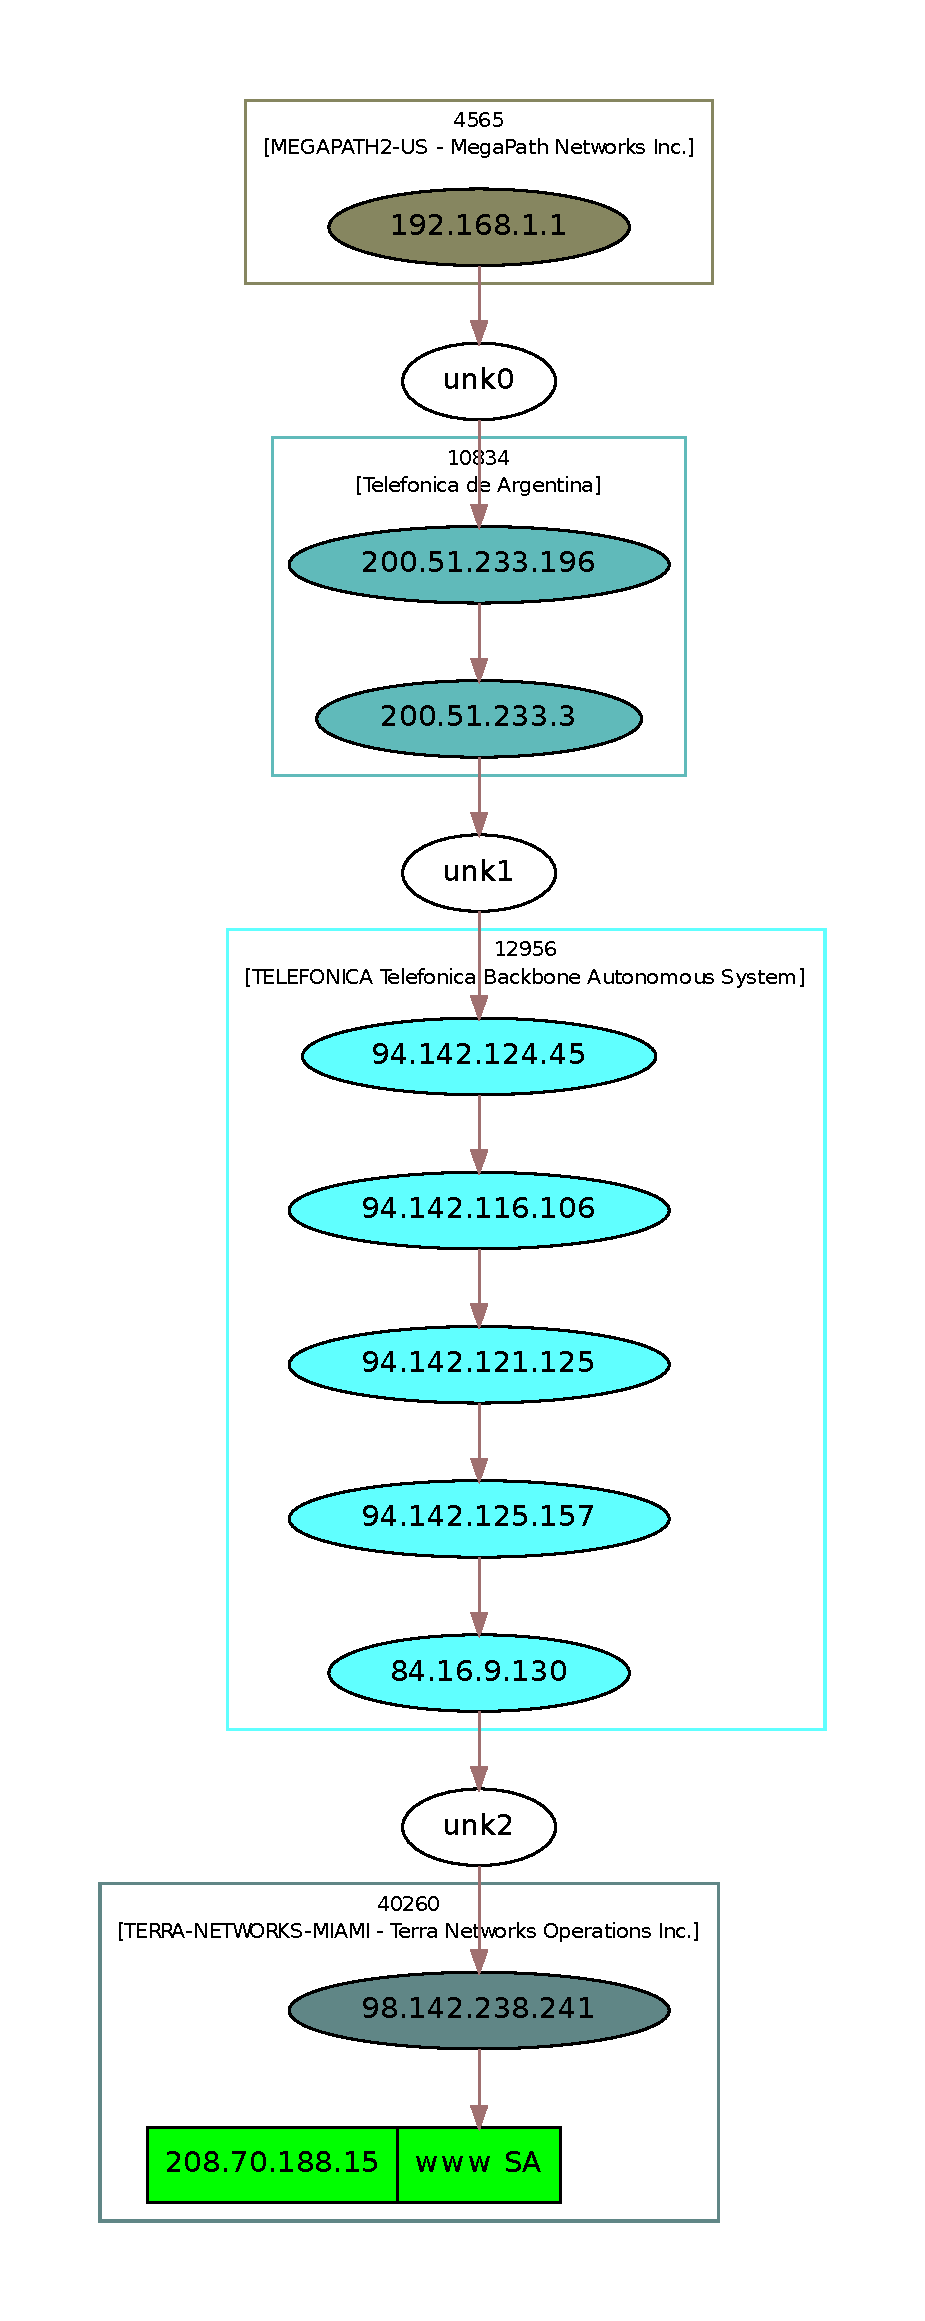
\includegraphics[width=0.4\textwidth]{./figs/ruta_google.pdf}
  \caption{Diagrama de una ruta trazada por $traceroute$ de Scapy}
\end{figure}

\newpage

%%%%%%%%%%%%%%%%%%%%
%    Desarrollo    				 %
%%%%%%%%%%%%%%%%%%%%

\section{Desarrollo}

\subsection{Elección de Destinos}

Para realizar los experimentos se eligieron 3 universidades de distintos continentes para así poder presentar variedad en las rutas examinadas y poder analizar, luego, cuánto impactan los enlaces transatlánticos. En el Cuadro~\ref{tab:infouniv} se muestra la información de dichos destinos. Para el cálculo teórico del \textit{RTT}, las distancias se estimaron entre ciudad origen de los experimentos (\textsl{Ciudad Autónoma de Buenos Aires, Argentina}) y las respectivas ciudades de las universidades destino. Para ello se utilizó la herramienta de cálculo implementada en \textit{GeoBytes} \footnote{http://www.geobytes.com/citydistancetool.htm}. En la figura~\ref{fig:mapuniv1} se graficaron en un mapa los respectivos puntos con una estimación gráfica de la distancia lineal entre ellos.\\

\begin{table}[h]
    \centering
    \begin{tabular}{ | c | c | c | c | c |}
	    \hline
	    \textbf{Universidad} & \textbf{URL} & \textbf{IP} & \textbf{Continente} & \textbf{Distancia \textit{(km)}}\\ \hline
	    Univ. de California, Berkeley & http://www.berkeley.edu & 169.229.216.200 & América & 10412\\ \hline
	    Univ. de Oxford & http://www.ox.ac.uk & 163.1.60.42 & Europa & 11107\\ \hline
	    Universidad de Tokio & http://www.u-tokyo.ac.jp & 59.106.161.11 & Asia & 18372\\ \hline
    \end{tabular}
    \caption{Información sobre Universidades destino elegidas.}
    \label{tab:infouniv}
\end{table}

\begin{figure}[h!]
  \centering
  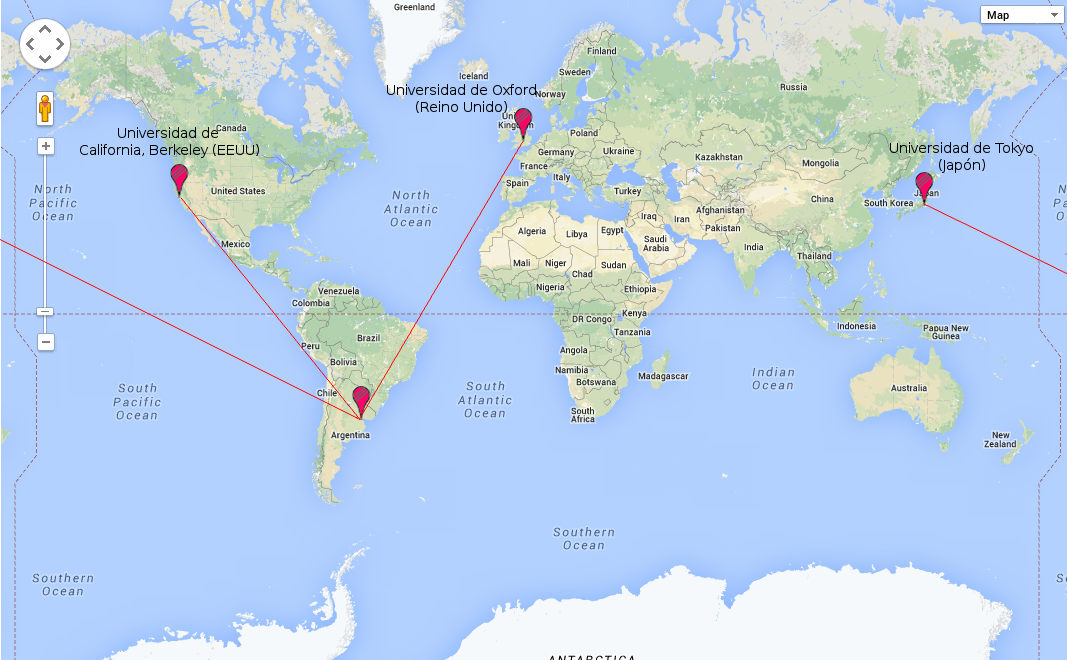
\includegraphics[width=0.7\textwidth]{./figs/map-univs1.png}
  \caption{Localización del origen y destinos con las respectivas distancias lineales aproximadas}
  \label{fig:mapuniv1}
\end{figure}

\subsection{Implementación de \textsl{Traceroute}}

El objetivo de la herramienta \textsl{traceroute} es examinar y trazar una porción de la ruta que atraviesa un paquete desde un origen hasta cierto destino a lo largo de las distintas redes por las que navega. Si bien tanto el sistema operativo Linux como la biblioteca de \textit{Python}, \textsl{Scapy}, proveen robustas implementaciones de esta utilidad, en principio no aplican para tomar tiempos, entre ellos el \textit{RTT}. Es por eso que se procedió a una implementación propia de \textsl{traceroute} basado en el enfoque de envío de paquetes \textit{ICMP}. En un \textit{ping} tradicional, dado un origen y un destino, el primero envía un paquete IP junto con un mensaje ICMP de tipo \textit{echo-request} a la espera de una respuesta satisfactoria de tipo \textit{echo-reply}. Para que esto suceda con éxito, el paquete ip debe tener un valor suficientemente grande en su campo \textit{ttl - time to live} de modo que los distintos nodos de la ruta lo reenvien hacia destino. En caso de que ese campo no sea suficiente para que el paquete llegue al destino deseado, el nodo que detecta el agotamiento de su \textit{ttl} responde con un mensaje ICMP de tipo {time-exceeded}. Tomando esta característica de la transmisión de paquetes y mensajes ICMP, la idea detrás de esta implementación de traceroute consiste en realizar sucesivos envíos de un paquete IP + mensaje ICMP \textit{echo-request} a destino comenzando con un \textit{ttl} unitario e incrementándolo en uno. De esta manera, el paquete 'muere' en distintos puntos del tramo y se puede identificar algunos de los nodos que se atraviesan ya que estos proveen su información al responder \textit{time-exceeded}.\\
\indent En el siguiente pseudocódigo se exhibe la idea detrás del algoritmo implementado.\\

\begin{algorithm}
\caption{traceroute (\textbf{in} $ipDest$, \textbf{in} $max\_hops$)}
\begin{algorithmic}[1]

\STATE $ttl \leftarrow 1$
\WHILE{$ttl < max\_hops$ y no se llego a destino}
	\STATE enviar mensaje ICMP \textsl{echo-request} sobre paquete IP con $ipDest$ y $ttl$
	\IF{hubo $respuesta$}
		\IF{$respuesta$ es de tipo \textsl{echo-reply}}
			\STATE imprimir datos de emisor de $respuesta$ y terminar
		\ELSE
			\STATE imprimir datos de emisor de $respuesta$
		\ENDIF
	\ENDIF
	\STATE $ttl \leftarrow ttl + 1$
\ENDWHILE
\end{algorithmic}
\end{algorithm}

\indent Al poder acceder al interior de este algoritmo, la modificación que se realizó fue la de realizar una diferencia de tiempo entre el instante previo al envío del mensaje y el instante posterior a la recepción de la respuesta. De esta manera, por cada paso de la ruta tenemos un valor empírico del $RTT$. Así podemos contar con todos los $round-trip$ $time$ de origen a cada nodo de la ruta y en particular a la de destino. En cierta forma esta versión de traceroute lleva implícita la funcionalidad de \textsl{ping}. Es importante notar que pueden existir valores de $ttl$ para los cuales no se obtenga respuesta (se supera el timeout del envío). Esto se puede deber a múltiples factores, pero no afecta la performance del algoritmo ya que se sigue adelante con un tiempo de vida mayor.\\

\subsection{Estimación de \textsl{RTT} empírico}

Basta con realizar un simple $ping$ a algún destino para notar a simple vista que los $round-trip$ $times$ empíricos son muy variables. Con el objetivo de obtener un valor algo más uniforme y representativo, exento de las particularidades temporales y espaciales de cada medición puntual, confeccionamos scripts para realizar $n$ mediciones de traceroute y poder volcar estos resultados en una matriz de datos. Por un lado, el script $rtt_traceroute$ de python toma un valor límite de $rtt$, una cantidad de iteraciones $n$ y un archivo de entrada con ternas de nombre, dns e ip de destino. Luego procede a ejecutar, para cada línea, $n$ iteraciones de traceroute, guardando el $rtt$ devuelto para el nodo final -destinatario- de la ruta. Por otro lado, el script en $Ruby$ lleva a cabo una tarea similar sólo que se vale de la herramienta 'traceroute' de Linux, la cual envía tres mensajes ICMP por valor de $ttl$, lo que totaliza 3 $rtt$ por cada ejecución. Finalmente, para procesar estos datos se crearon scripts de $Octave$ mediante los cuales se pudiera importar las matrices de resultados y realizar un promedio de los $round-trip$ $time$ para luego graficarlos en los diversos resultados presentados. Dependiendo de los experimentos la metodología puede haber variado un poco, caso en el cual se ampliará en la sección de Análisis.

\subsection{Detección de Enlaces Transatlánticos}

Con el fin de identificar posibles enlaces transatlánticos se creó el programa $trans\_atlantic\_traceroute$ en $Python$ que, dada la ruta con sus respectivos $rtt$ calculada por el algoritmo anterior, aplica la heurística recomendada en la consigna del trabajo para separar los posibles hops involucrados en un enlace del tipo buscado.


\clearpage

%%%%%%%%%%%%%%%%%%%%
%    Resultados    				 %
%%%%%%%%%%%%%%%%%%%%

\section{Resultados}
\clearpage

%%%%%%%%%%%%%%%%%%%
%    Discusión    			   %
%%%%%%%%%%%%%%%%%%%

\section{Análisis}

\subsection{RTT por ciudad}

Se realizaron varias pruebas en distintos horarios del día contra las distintas universidades, para determinar si hay o no una diferencia en performance de la conexión según la cantidad de carga del host al que nos conectamos.\\
\\
\indent Nuestra hipótesis era que según en que momento del día nos conectemos, mejora o empeora el \textit{roundtrip time} según que tanto uso se le esté dando en el momento a las conexiones. Pasamos a verificar esto empíricamente.\\
\\
\indent Con este fin, determinamos distintas franjas horarias que creímos representativas de distintos momentos del día. Las mismas son: \textbf{00hs, 02hs, 08hs, 11hs, 15hs, 22hs}

\subsubsection{Universidad de Tokio}
Empezaremos explicando el más inmediato, que es el resultado de la Universidad de Tokio. Como se puede ver en la figura~\ref{fig:rtt-horarios-tokyo}, es marcada la diferencia de tiempo que nos toma enviar algo y recibir una respuesta entre las 2am y las 3pm nuestras, que equivalen a las 2pm y las 3am de ellos.\\
\indent Podemos apreciar que a las 3am el roundtrip time puede bajar hasta más de la mitad que el visto a las 2pm, momento en el que es mucho más probable que haya gente en la facultad utilizando los equipos y la red.

\subsubsection{Universidad de California}
En la figura~\ref{fig:rtt-horarios-california} se pueden ver los resultados obtenidos para la Universidad de Berkeley, California. Su huso horario acusa 4hs menos que el de Argentina, por lo tanto, las franjas más diferenciadas son las 7am y 6pm.\\
\indent Este resultado es un poco más ambiguo, mostrando cierta estabilidad a las 7am con un RTT que está alrededor de los 240ms casi siempre, y un comportamiento más disperso a las 6pm, momento en el cual se ven resultados un poco peores (entre 320 y 520ms, aproximadamente), y otros un poco mejores (cerca de los 180 o 200ms). Ambos horarios nos parecen coherentes para que la Universidad tenga sus equipos en uso, y las demás franjas horarias no mostraron mayores variaciones, sino que se manejaban entre estos valores.

\subsubsection{Universidad de Oxford}
Finalmente vemos que pasa con las conexiones a la Universidad de Oxford, cuyo horario es 4hs agregadas al nuestro. Los resultados más significativos resultaron ser los de las 3pm y las 10pm, que representan las 7pm y 2am locales.\\
\indent Uno esperaría un resultado similar al de Tokio, en el cual por la madrugada la carga era menor y el RTT, por ende, también. La figura~\ref{fig:rtt-horarios-oxford} nos muestra que no es tan así, sino que en la franja de las 7pm hay un desempeño mucho más estable que en el de las 2am. Dicho desempeño no sólo es más estable, sino que también es mejor (menos RTT en general). Desconocemos las causas de por qué puede estar pasando esto.

\newpage

%%%%%%%%%%%%%%%%%%%%%%
%    Conclusiones   				 %
%%%%%%%%%%%%%%%%%%%%%%

\section{Conclusiones}

Luego de hacer las pruebas hacia distintas partes del mundo y en distintos horarios para calcular el RTT, podemos concluir que nuestra hipótesis (mencionada en el apartado \textbf{4.1}) en gran parte se cumple, pero no siempre. Podemos ver que en varios momentos (sobretodo en la prueba contra Tokio) tiene sentido, pero para obtener un mayor grado de precisión, habría que realizar a futuro más experimentos durante una mayor cantidad de tiempo y, tal vez, en otras franjas horarias para sacar conclusiones más precisas con respecto a lo que pasa realmente.
\newpage

%%%%%%%%%%%%%%%%%%%
%    Apéndices    			   %
%%%%%%%%%%%%%%%%%%%

\section{Apéndices}
\newpage

%%%%%%%%%%%%%%%%%%%%%
%    Referencias 				   %
%%%%%%%%%%%%%%%%%%%%%

\section{Referencias}
\newpage



















%%%%%%%%%%%%%%%%%%%%%%%%%%%%%%%%%%%%%%%%
%        Esto es de mi template        %
%    Dejar para futuras referencias    %
%%%%%%%%%%%%%%%%%%%%%%%%%%%%%%%%%%%%%%%%

% \section{Sección, título grande}
% \\
% \textcolor{white}{Sarasa engañadora de formato, jua jua}\\
% Esto es texto. Con doble barra invertida es el enter.
% \\
% \\
% \textit{De acá en adelante, todo lo que se explica como "para hacer x se usa y", implica que antes de y va una barra invertida}
% \\
% \\
% Con \textbf{textbf\{\}} se escribe en negrita.
% \\
% \\
% \section{Bullet \& Numbering}
% Para hacer items se usa \textbf{begin\{itemize\}} y \textbf{end\{itemize\}}, por ejemplo:
% \begin{itemize}
% 	\item Esto es un ítem.
% 	\item Esto es otro.
% \end{itemize}
% Con \textbf{item} se hace cada uno de los ítems. Si cambiás \textbf{itemize} por \textbf{enumerate} te lo hace enumerado. Por ejemplo:
% \begin{enumerate}
% 	\item Acá está el primero.
% 	\item Acá el segundo.
% \end{enumerate}
% \\
% Y así.
% \\
% \\
% \section{Tablas}
% También tenemos las tablas, que son un poco más rebuscadas. Se usa \textbf{begin\{tabular\}\{cols\}} y en cols ponemos c si queremos una columna centrada, l y r
% para otro tipo de justificación. Si las c las separás con espacios, se hacen columnas sin división. Si ponés un pipe es con una línea divisoria, dos pipes con
% dos líneas, y así. Se termina con \textbf{end\{tabular\}}. Para separar entre elementos de fila/columna se usa un ampersand (\&, y es necesario para separar
% elementos entre filas y columnas, no solo entre filas) y para cambiar de fila \textbf{SIN} linea divisoria, un \textbf{newline} ya que el doble barra invertida
% te hace un enter dentro de la celda. Con línea divisoria es reemplazando \textbf{newline} por \textbf{hline}.
% \\
% \\
% Más datos en el principio de este tex. Un ejemplo:
% \\
% \\
% \begin{tabular}{| c| c|}\hline
%     Celda 1 & Celda 2 &\hline
%     Celda 3 & Celda 4 &\hline
% \end{tabular}
% \\
% \\
% \section{Verbatim}
% \begin{verbatim}
% Esto es verbatim. Es un entorno que no le da ni 5 de pelota al formato de latex.
% Por eso mismo hay que tener cuidado con no irse de la hoja o similar.
% Sirve por ejemplo, para pseudocódigo:
% 
% if (se cumple sarasa){
%     ejecuto cosito1;
%     ejecuto cosito2:
% }else{
%     ejecuto cosito3:
% }
% \end{verbatim}

\end{document}
